\documentclass[journal,12pt,twocolumn]{IEEEtran}
%
\usepackage{setspace}
\usepackage{gensymb}
\singlespacing
\usepackage[cmex10]{amsmath}
\usepackage{siunitx}
\usepackage{amsthm}

\usepackage{mathrsfs}

\usepackage{txfonts}
\usepackage{stfloats}

\usepackage{steinmetz}
\usepackage{cite}
\usepackage{cases}
\usepackage{subfig}
\usepackage{longtable}
\usepackage{multirow}
\usepackage{enumitem}
\usepackage{mathtools}
\usepackage{tikz}
\usepackage{circuitikz}
\usepackage{verbatim}
\usepackage{tfrupee}
\usepackage[breaklinks=true]{hyperref}
\usepackage{tkz-euclide} % loads  TikZ and tkz-base
\usetikzlibrary{calc,math}
\usetikzlibrary{fadings}
\usepackage{listings}
    \usepackage{color}                                            %%
    \usepackage{array}                                            %%
    \usepackage{longtable}                                        %%
    \usepackage{calc}                                             %%
    \usepackage{multirow}                                         %%
    \usepackage{hhline}                                           %%
    \usepackage{ifthen}                                           %%
  %optionally (for landscape tables embedded in another document): %%
    \usepackage{lscape}     
\usepackage{multicol}
\usepackage{chngcntr}
\DeclareMathOperator*{\Res}{Res}

\renewcommand\thesection{\arabic{section}}
\renewcommand\thesubsection{\thesection.\arabic{subsection}}
\renewcommand\thesubsubsection{\thesubsection.\arabic{subsubsection}}

\renewcommand\thesectiondis{\arabic{section}}
\renewcommand\thesubsectiondis{\thesectiondis.\arabic{subsection}}
\renewcommand\thesubsubsectiondis{\thesubsectiondis.\arabic{subsubsection}}

\hyphenation{op-tical net-works semi-conduc-tor}
\def\inputGnumericTable{}                                 %%

\lstset{
%language=C,
frame=single, 
breaklines=true,
columns=fullflexible
}
\begin{document}
%


\newtheorem{theorem}{Theorem}[section]
\newtheorem{problem}{Problem}
\newtheorem{proposition}{Proposition}[section]
\newtheorem{lemma}{Lemma}[section]
\newtheorem{corollary}[theorem]{Corollary}
\newtheorem{example}{Example}[section]
\newtheorem{definition}[problem]{Definition}
\newcommand{\BEQA}{\begin{eqnarray}}
\newcommand{\EEQA}{\end{eqnarray}}
\newcommand{\define}{\stackrel{\triangle}{=}}
\bibliographystyle{IEEEtran}
\providecommand{\mbf}{\mathbf}
\providecommand{\pr}[1]{\ensuremath{\Pr\left(#1\right)}}
\providecommand{\qfunc}[1]{\ensuremath{Q\left(#1\right)}}
\providecommand{\sbrak}[1]{\ensuremath{{}\left[#1\right]}}
\providecommand{\lsbrak}[1]{\ensuremath{{}\left[#1\right.}}
\providecommand{\rsbrak}[1]{\ensuremath{{}\left.#1\right]}}
\providecommand{\brak}[1]{\ensuremath{\left(#1\right)}}
\providecommand{\lbrak}[1]{\ensuremath{\left(#1\right.}}
\providecommand{\rbrak}[1]{\ensuremath{\left.#1\right)}}
\providecommand{\cbrak}[1]{\ensuremath{\left\{#1\right\}}}
\providecommand{\lcbrak}[1]{\ensuremath{\left\{#1\right.}}
\providecommand{\rcbrak}[1]{\ensuremath{\left.#1\right\}}}
\theoremstyle{remark}
\newtheorem{rem}{Remark}
\newcommand{\sgn}{\mathop{\mathrm{sgn}}}
\providecommand{\abs}[1]{\left\vert#1\right\vert}
\providecommand{\abs}[1]{\lvert#1\rvert} 
\providecommand{\res}[1]{\Res\displaylimits_{#1}} 
\providecommand{\norm}[1]{\left\lVert#1\right\rVert}
%\providecommand{\norm}[1]{\lVert#1\rVert}
\providecommand{\mtx}[1]{\mathbf{#1}}
\providecommand{\mean}[1]{E\left[ #1 \right]}
\providecommand{\fourier}{\overset{\mathcal{F}}{ \rightleftharpoons}}
%\providecommand{\hilbert}{\overset{\mathcal{H}}{ \rightleftharpoons}}
\providecommand{\system}{\overset{\mathcal{H}}{ \longleftrightarrow}}
	%\newcommand{\solution}[2]{\textbf{Solution:}{#1}}
\newcommand{\solution}{\noindent \textbf{Solution: }}
\newcommand{\cosec}{\,\text{cosec}\,}
\providecommand{\dec}[2]{\ensuremath{\overset{#1}{\underset{#2}{\gtrless}}}}
\newcommand{\myvec}[1]{\ensuremath{\begin{pmatrix}#1\end{pmatrix}}}
\newcommand{\mydet}[1]{\ensuremath{\begin{vmatrix}#1\end{vmatrix}}}
\numberwithin{equation}{subsection}
\makeatletter
\@addtoreset{figure}{problem}
\makeatother
\let\StandardTheFigure\thefigure
\let\vec\mathbf
\renewcommand{\thefigure}{\theproblem}
\def\putbox#1#2#3{\makebox[0in][l]{\makebox[#1][l]{}\raisebox{\baselineskip}[0in][0in]{\raisebox{#2}[0in][0in]{#3}}}}
     \def\rightbox#1{\makebox[0in][r]{#1}}
     \def\centbox#1{\makebox[0in]{#1}}
     \def\topbox#1{\raisebox{-\baselineskip}[0in][0in]{#1}}
     \def\midbox#1{\raisebox{-0.5\baselineskip}[0in][0in]{#1}}
\vspace{3cm}
\title{ASSIGNMENT-6}
\author{R.YAMINI}
\maketitle
\newpage
\bigskip
\renewcommand{\thefigure}{\theenumi}
\renewcommand{\thetable}{\theenumi}


%
\section{QUESTION No-2.82 (Quadratic forms)}
\item Find the equation of the tangent to the curve $y=\sqrt{3x-2}$ which is parallel to the line $\myvec{4&-2}\vec{x} + 5 = 0$.

%

\section{Solution}
Given equation
\begin{align}
    \vec{x}^{\top}\myvec{0&0 \\ 0&1}\vec{x}+\myvec{-3&0}\vec{x}+2=0 \label{eq:giveneq}
\end{align}
we have 
\begin{align}
\therefore \vec{u}=\myvec{\frac{-3}{2} \\ 0}
\\
\vec{V} =\myvec{0&0 \\ 0&1}
\\
\implies \mymacro{\mydet{\vec{V}}}=0
\end{align}
Thus the curve is a parabola.Now we find the eigen values corresponding to $\vec{V}$
\begin{align}
    \mydet{\vec{V}-\lambda\vec{I}} = 0
    \\
    \mydet{-\lambda&0 \\ 0&1-\lambda}=0
    \\
    \implies \lambda= 0,1
\end{align}
Now we find the eigen vectors corresponding to $\lambda= 0,1$ respectively.
\begin{align}
    \vec{V}\vec{x} = \lambda\vec{x}
    \\
    \myvec{0&0 \\ 0&1}\vec{x} = 0\implies \vec{p_{1}}= \myvec{1 \\ 0}
    \\
    \myvec{-1&0 \\ 0&0}\vec{x} = \vec{x}\implies \vec{p_{2}}= \myvec{0 \\ 1}
\end{align}
Now by eigen decomposition on $\vec{V}$
\begin{align}
    \vec{V} = \vec{P}\vec{D}\vec{P}^{\top}\label{eq:eqn1}
\end{align}
where 
\begin{align}
 \vec{P} = \brak{\vec{p_{1}}\vec{p_{2}}} = \myvec{1&0 \\ 0&1}
 \\
 \vec{D}=\myvec{\lambda_{1}&0 \\ 0&\lambda_{2}} = \myvec{0&0 \\ 0&1}
\end{align}
Now \eqref{eq:eqn1} becomes
\begin{align}
    \vec{V}=\myvec{1&0 \\ 0&1}\myvec{0&0 \\ 0&1}\myvec{1&0 \\ 0&1}
    \\
    \vec{V}=\myvec{0&0 \\ 0&1}
\end{align}
Given parallel line equation 
\begin{align}
 \myvec{4&-2}\vec{x} + 5 = 0\label{eq:eqn2}
\end{align}
Now the tangent to the parabola is parallel to the line equation \eqref{eq:eqn2},
The normal vector $\vec{n}$ and the direction vector $\vec{m}$ is given by 
\begin{align}
    \vec{n}=\myvec{4 \\ -2} \label{eq:eqn5}
    \\
    \vec{m}=\myvec{-2 \\ -4}
\end{align}
Now the equation for the point of contact for the parabola is given as,
\begin{align}
    \myvec{\vec{u}+\kappa \vec{n}^{\top} \\ \vec{V} }\vec{q} &= \myvec{\vec{-f}\\\kappa \vec{n} -\vec{u}}
    \\
    \kappa =\frac{\vec{p_{1}}^{\top}\vec{u}}{\vec{p_{1}}^{\top}\vec{n}}
    =\frac{\myvec{1&0}\myvec{\frac{-3}{2} \\ 0}}{\myvec{1&0}\myvec{4 \\ 2}}
    =\frac{-3}{8}
    \\
   \implies\myvec{-3&\frac{3}{4} \\ 0&0 \\ 0&1} \vec{q}&= \myvec{-2 \\ 0 \\ \frac{3}{4}}
\end{align}
Now solving for $\vec{q}$ by removing the zero row and representing as augmented matrix and then converting it to echelon form.
\begin{align}
    \myvec{-3&\frac{3}{4}&-2 \\ 0&1&\frac{3}{4}}\xleftrightarrow{R_1\rightarrow \brak{\frac{-1}{3}}R_1} \myvec{1&\frac{-1}{4}&\frac{2}{3} \\ 0&1&\frac{3}{4}}
    \\
    \myvec{1&\frac{-1}{4}&\frac{2}{3} \\ 0&1&\frac{3}{4}}\xleftrightarrow{R_1\rightarrow R_1+\frac{1}{4}R_2}\myvec{1&0&\frac{41}{48} \\ 0&1&\frac{3}{4}} \label{eq:eqn3}
\end{align}
Hence from the \eqref{eq:eqn3} we get the point of contact to be 
\begin{align}
    \vec{q}=\myvec{\frac{41}{48} \\ \frac{3}{4}}
\end{align}
Now $\vec{q}$ is the point on the tangent.Hence the equation of the line can be expressed as 
\begin{align}
    \mathbf{n}^{\top}(\mathbf{x}-\mathbf{q}) = 0\label{eq:eqn6}
\end{align}
where,
\begin{align}
\vec{n}^{\top}\vec{q}
    =\myvec{4&-2}\myvec{\frac{41}{48} \\ \frac{3}{4}} 
    \\
    = \frac{23}{12} \label{eq:eqn4}
\end{align}
Hence the equation of the tangent to the curve \eqref{eq:giveneq} parallel to the line \eqref{eq:eqn2} is given by substituting the value of $\vec{n}^{\top}\vec{q}$ and $\vec{n}$ from \eqref{eq:eqn4} and \eqref{eq:eqn5} respectively to the equation \eqref{eq:eqn6} 
\begin{align}
    \myvec{4&-2}\vec{x}=\frac{23}{12} \label{eq:eqn7}
\end{align}
Hence \eqref{eq:eqn7} is the equation of the tangent.
The plot of the figure is given below

\numberwithin{figure}{section}
\begin{figure}[ht]
\centering
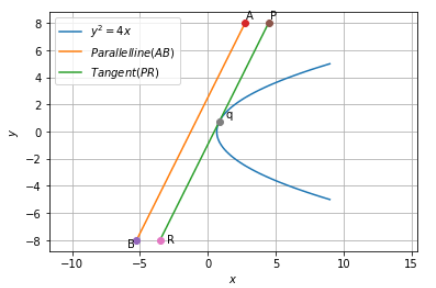
\includegraphics[width=\columnwidth]{Parabola.PNG}
\caption{Plot of curve and the lines}
\label{Plot of curve and the lines}
\end{figure}
\end{document}
